% Options for packages loaded elsewhere
\PassOptionsToPackage{unicode}{hyperref}
\PassOptionsToPackage{hyphens}{url}
\PassOptionsToPackage{dvipsnames,svgnames,x11names}{xcolor}
%
\documentclass[
  letterpaper,
  DIV=11,
  numbers=noendperiod,
  oneside]{scrartcl}

\usepackage{amsmath,amssymb}
\usepackage{iftex}
\ifPDFTeX
  \usepackage[T1]{fontenc}
  \usepackage[utf8]{inputenc}
  \usepackage{textcomp} % provide euro and other symbols
\else % if luatex or xetex
  \usepackage{unicode-math}
  \defaultfontfeatures{Scale=MatchLowercase}
  \defaultfontfeatures[\rmfamily]{Ligatures=TeX,Scale=1}
\fi
\usepackage{lmodern}
\ifPDFTeX\else  
    % xetex/luatex font selection
\fi
% Use upquote if available, for straight quotes in verbatim environments
\IfFileExists{upquote.sty}{\usepackage{upquote}}{}
\IfFileExists{microtype.sty}{% use microtype if available
  \usepackage[]{microtype}
  \UseMicrotypeSet[protrusion]{basicmath} % disable protrusion for tt fonts
}{}
\makeatletter
\@ifundefined{KOMAClassName}{% if non-KOMA class
  \IfFileExists{parskip.sty}{%
    \usepackage{parskip}
  }{% else
    \setlength{\parindent}{0pt}
    \setlength{\parskip}{6pt plus 2pt minus 1pt}}
}{% if KOMA class
  \KOMAoptions{parskip=half}}
\makeatother
\usepackage{xcolor}
\usepackage[left=1in,marginparwidth=2.0666666666667in,textwidth=4.1333333333333in,marginparsep=0.3in]{geometry}
\setlength{\emergencystretch}{3em} % prevent overfull lines
\setcounter{secnumdepth}{5}
% Make \paragraph and \subparagraph free-standing
\makeatletter
\ifx\paragraph\undefined\else
  \let\oldparagraph\paragraph
  \renewcommand{\paragraph}{
    \@ifstar
      \xxxParagraphStar
      \xxxParagraphNoStar
  }
  \newcommand{\xxxParagraphStar}[1]{\oldparagraph*{#1}\mbox{}}
  \newcommand{\xxxParagraphNoStar}[1]{\oldparagraph{#1}\mbox{}}
\fi
\ifx\subparagraph\undefined\else
  \let\oldsubparagraph\subparagraph
  \renewcommand{\subparagraph}{
    \@ifstar
      \xxxSubParagraphStar
      \xxxSubParagraphNoStar
  }
  \newcommand{\xxxSubParagraphStar}[1]{\oldsubparagraph*{#1}\mbox{}}
  \newcommand{\xxxSubParagraphNoStar}[1]{\oldsubparagraph{#1}\mbox{}}
\fi
\makeatother


\providecommand{\tightlist}{%
  \setlength{\itemsep}{0pt}\setlength{\parskip}{0pt}}\usepackage{longtable,booktabs,array}
\usepackage{calc} % for calculating minipage widths
% Correct order of tables after \paragraph or \subparagraph
\usepackage{etoolbox}
\makeatletter
\patchcmd\longtable{\par}{\if@noskipsec\mbox{}\fi\par}{}{}
\makeatother
% Allow footnotes in longtable head/foot
\IfFileExists{footnotehyper.sty}{\usepackage{footnotehyper}}{\usepackage{footnote}}
\makesavenoteenv{longtable}
\usepackage{graphicx}
\makeatletter
\newsavebox\pandoc@box
\newcommand*\pandocbounded[1]{% scales image to fit in text height/width
  \sbox\pandoc@box{#1}%
  \Gscale@div\@tempa{\textheight}{\dimexpr\ht\pandoc@box+\dp\pandoc@box\relax}%
  \Gscale@div\@tempb{\linewidth}{\wd\pandoc@box}%
  \ifdim\@tempb\p@<\@tempa\p@\let\@tempa\@tempb\fi% select the smaller of both
  \ifdim\@tempa\p@<\p@\scalebox{\@tempa}{\usebox\pandoc@box}%
  \else\usebox{\pandoc@box}%
  \fi%
}
% Set default figure placement to htbp
\def\fps@figure{htbp}
\makeatother

\usepackage{endnotes}
\let\footnote=\endnote
\KOMAoption{captions}{tableheading}
\makeatletter
\@ifpackageloaded{tcolorbox}{}{\usepackage[skins,breakable]{tcolorbox}}
\@ifpackageloaded{fontawesome5}{}{\usepackage{fontawesome5}}
\definecolor{quarto-callout-color}{HTML}{909090}
\definecolor{quarto-callout-note-color}{HTML}{0758E5}
\definecolor{quarto-callout-important-color}{HTML}{CC1914}
\definecolor{quarto-callout-warning-color}{HTML}{EB9113}
\definecolor{quarto-callout-tip-color}{HTML}{00A047}
\definecolor{quarto-callout-caution-color}{HTML}{FC5300}
\definecolor{quarto-callout-color-frame}{HTML}{acacac}
\definecolor{quarto-callout-note-color-frame}{HTML}{4582ec}
\definecolor{quarto-callout-important-color-frame}{HTML}{d9534f}
\definecolor{quarto-callout-warning-color-frame}{HTML}{f0ad4e}
\definecolor{quarto-callout-tip-color-frame}{HTML}{02b875}
\definecolor{quarto-callout-caution-color-frame}{HTML}{fd7e14}
\makeatother
\makeatletter
\@ifpackageloaded{caption}{}{\usepackage{caption}}
\AtBeginDocument{%
\ifdefined\contentsname
  \renewcommand*\contentsname{Table of contents}
\else
  \newcommand\contentsname{Table of contents}
\fi
\ifdefined\listfigurename
  \renewcommand*\listfigurename{List of Figures}
\else
  \newcommand\listfigurename{List of Figures}
\fi
\ifdefined\listtablename
  \renewcommand*\listtablename{List of Tables}
\else
  \newcommand\listtablename{List of Tables}
\fi
\ifdefined\figurename
  \renewcommand*\figurename{Figure}
\else
  \newcommand\figurename{Figure}
\fi
\ifdefined\tablename
  \renewcommand*\tablename{Table}
\else
  \newcommand\tablename{Table}
\fi
}
\@ifpackageloaded{float}{}{\usepackage{float}}
\floatstyle{ruled}
\@ifundefined{c@chapter}{\newfloat{codelisting}{h}{lop}}{\newfloat{codelisting}{h}{lop}[chapter]}
\floatname{codelisting}{Listing}
\newcommand*\listoflistings{\listof{codelisting}{List of Listings}}
\makeatother
\makeatletter
\makeatother
\makeatletter
\@ifpackageloaded{caption}{}{\usepackage{caption}}
\@ifpackageloaded{subcaption}{}{\usepackage{subcaption}}
\makeatother
\makeatletter
\@ifpackageloaded{sidenotes}{}{\usepackage{sidenotes}}
\@ifpackageloaded{marginnote}{}{\usepackage{marginnote}}
\makeatother

\usepackage[]{natbib}
\bibliographystyle{plainnat}
\usepackage{bookmark}

\IfFileExists{xurl.sty}{\usepackage{xurl}}{} % add URL line breaks if available
\urlstyle{same} % disable monospaced font for URLs
\hypersetup{
  pdftitle={Step by step guide on how to ruin your company and your team with AI},
  colorlinks=true,
  linkcolor={blue},
  filecolor={Maroon},
  citecolor={Blue},
  urlcolor={Blue},
  pdfcreator={LaTeX via pandoc}}


\title{Step by step guide on how to ruin your company and your team with
AI}
\usepackage{etoolbox}
\makeatletter
\providecommand{\subtitle}[1]{% add subtitle to \maketitle
  \apptocmd{\@title}{\par {\large #1 \par}}{}{}
}
\makeatother
\subtitle{A roadmap to the quickest way to lose your team's trust}
\author{}
\date{2025-02-12}

\begin{document}
\maketitle


It's pretty easy to keep a team organized with a well-defined workflow,
right?

But if you want to showcase your incompetence or simply watch everything
go up in flames, this post is for you!

Already in a leadership position and ready to swim against the tide?
Here are some tips to quickly turn everything upside down, bringing
chaos and demotivation as fast as possible to everyone relying on your
work.

And the best part:

\begin{itemize}
\tightlist
\item
  Without much effort;
\item
  Reducing your workload;
\item
  And with the most groundbreaking tool of the moment\footnote{Generative
    Artificial Intelligence}!
\end{itemize}

To better understand where you can fail and make it blatantly obvious to
everyone, let's break down the following workflow I've created:

\pandocbounded{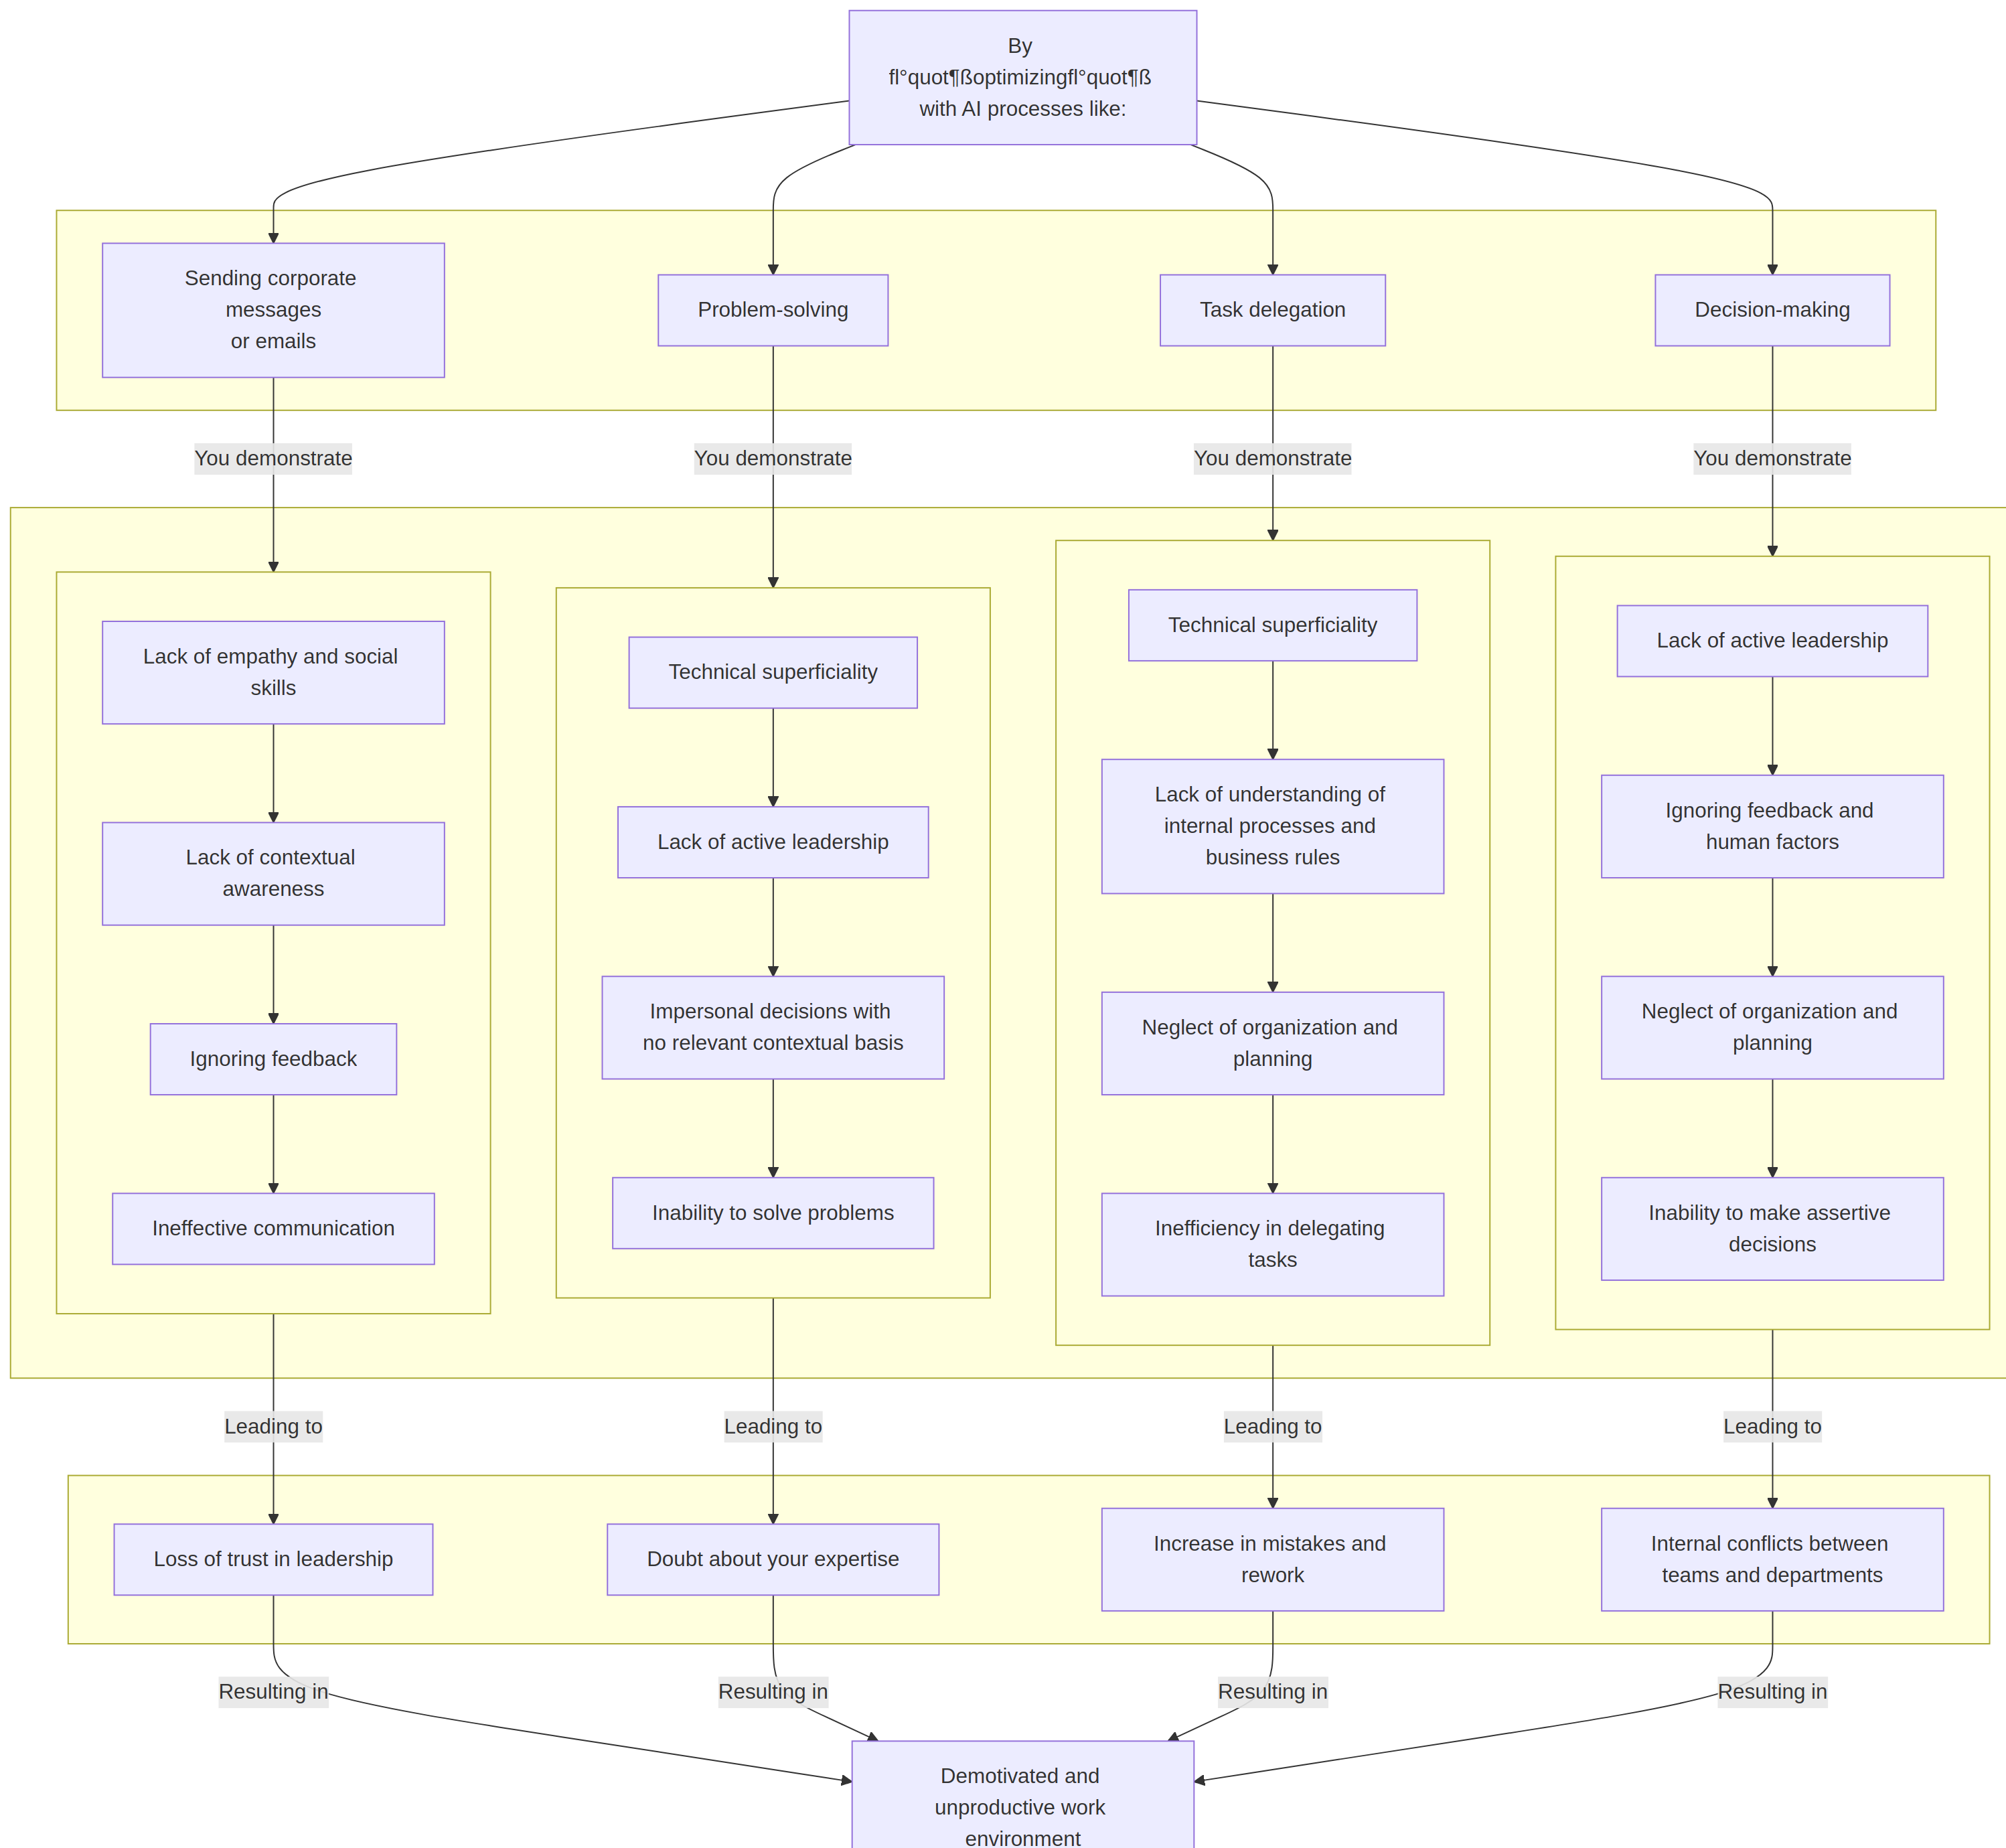
\includegraphics[keepaspectratio]{index_files/figure-latex/mermaid-figure-1.png}}

See how easy it is to visualize how simple processes can trigger a chain
of problems that will inevitably lead to your undeniable exclusion and
eventual termination?

Maybe you felt personally attacked by how this topic was introduced.

If so, part of that is due to the Psychological Reactance
phenomenon\footnote{See more at
  \citet{UnderstandingPsychologicalReactance}} combined with elements of
Reverse Psychology\footnote{See more at
  \citet{HowDoesReversePsychologyWork}}.

By deliberately exaggerating the impact of the indiscriminate use of
this miraculous tool\footnote{Generative Artificial Intelligence} ---
framing as ``correct'' something that is generally frowned upon---you,
as the likely target audience, are naturally inclined to resist and deny
it. After all, how hard is it to admit that what currently makes you a
professional could easily be the nightmare of many of your colleagues?
Or worse, that you could be replaced by an inanimate tool?

This negative reaction from this category of workers is expected since
they are already dependent on this enabler\footnote{Generative
  Artificial Intelligence}, and the idea that it might be harmful---not
just to them but to everyone around them---doesn't fit the short-term
results they have experienced so far.

From a broader perspective, part of the blame may not be entirely yours
but rather the fault of those who sold you the idea that this
tool\footnote{Generative Artificial Intelligence} is the solution to all
your monotonous tasks. However, the lack of supervision and limitation
of its use will always lead to its application in a wide range of
areas---without proper impact assessment and consideration of
consequences---far beyond the monotonous tasks it was originally
designed for\footnote{Generative Artificial Intelligence}.

Currently, most AI models are in constant development and far from their
peak, with limitations and flaws that are imperceptible at first glance.
This is because their entire functioning is designed to socially please
the user, meaning they are structured in a way that prevents you from
feeling like you're facing incorrect or nonsensical information.

Not convinced? Maybe you're still caught in Automation Bias\footnote{See
  more at \citet{DoesAutomationBiasDecisionMaking}}. To open your eyes,
here are some phenomena that might be happening to you daily without you
even realizing it:

\begin{itemize}
\tightlist
\item
  \textbf{Hallucinations}\footnote{See more at
    \citet{WhatAreAIHallucinations}}, where the tool\footnote{Generative
    Artificial Intelligence} generates responses that, while appearing
  coherent, have no real basis, being merely a statistical
  approximation\footnote{Which may result in an incorrect weight
    distribution} of what would best fit the given context. This happens
  due to the lack of logical reasoning in these products\footnote{Generative
    artificial intelligences}, making some responses essentially just
  ``educated guesses.''
\item
  \textbf{Context Window}\footnote{See more at
    \citet{WhatIsAContextWindow}}, which limits the amount of
  information the tool\footnote{Generative Artificial Intelligence} can
  process at once, meaning that it often fails to grasp the full context
  of a situation, leading to responses that don't align with reality.
  This becomes even more concerning as there is no explicit indication
  of what is or isn't discarded by the tool\footnote{Generative
    Artificial Intelligence}.
\end{itemize}

In conclusion, the use of AI tools in corporate environments should be
approached with caution and always under the supervision of a qualified
professional. After all, no tool can replace critical thinking and
assertive decision-making---no matter how convincing or convenient it
may seem.

I hope this reading has helped you open your eyes to the dangers of
so-called ``miracle'' automation tools, both for current AI and for
future technologies that may emerge.

\begin{tcolorbox}[enhanced jigsaw, bottomtitle=1mm, toptitle=1mm, opacityback=0, titlerule=0mm, colframe=quarto-callout-tip-color-frame, colbacktitle=quarto-callout-tip-color!10!white, toprule=.15mm, breakable, bottomrule=.15mm, left=2mm, title=\textcolor{quarto-callout-tip-color}{\faLightbulb}\hspace{0.5em}{Remember}, arc=.35mm, rightrule=.15mm, coltitle=black, opacitybacktitle=0.6, colback=white, leftrule=.75mm]

The problem is never the tool itself, but how it is used!

\end{tcolorbox}

\newpage
\theendnotes


  \bibliography{bibliography.bib}



\end{document}
